\documentclass{beamer}
\mode<presentation> {
\usetheme{CambridgeUS}
}
%\usecolortheme[named=blue]{structure}

\usepackage{color}
\usepackage{graphicx} % Allows including images
%	TITLE PAGE
\title[Department of Mathematics]{Pricing European down-and-out call options: an application to Vietnamese financial derivatives market}
\institute[] 
{\textbf{Department of Mathematics\\
International University, Vietnam National University} \\
\medskip
	\begin{figure}[htp]
	\begin{center}
		
\includegraphics[scale=.2]{logo}
	\end{center}
	\label{reflogo}
\end{figure}

\text{Author: Ta Thi Phuong Dung} \\
\text{Advisor: Dr. Le Nhat Tan} 
}
\date{\today}

\begin{document}

\begin{frame}
\titlepage 
\end{frame}
\begin{frame}
\frametitle{Outline} 
\tableofcontents
\end{frame}

\section{Introdution}
\begin{frame}
\begin{figure}[htp]
	\begin{center}
		
\includegraphics[scale=0.6]{PS}
	\end{center}
\end{figure}
\begin{itemize}
	\item On August 10, 2017, the VN30-Index futures contract were officially traded in the Vietnam market
	\item Options is a important type of financial derivatives products \\[0.3cm]
	\item Barrier options are very popular\\[0.3cm]
   \item Deriving the pricing formula using  probabilistic approach
\end{itemize}
\end{frame}

%------------------------------------------------
\section{The formula's derivation}
\begin{frame}
\frametitle{Option price}
\begin{figure}[htp]
	\begin{center}
		
\includegraphics[scale=0.6]{fig9}
	\end{center}
\begin{center}
	
\includegraphics[scale=0.6]{fig10}
\end{center}
\end{figure}	
\end{frame}
\begin{frame}
\frametitle{Pricing option procedure}
Option price at expiry is known from definition
\begin{align}
	C_{d/o}(S_T, T)=\max\{S_T-K, 0\}\mathcal{I}_{\underset{t\leq u\leq T}\min S_u > B}
\end{align}
The stock price $S_t$ follows a Geometric Brownian motion:
\begin{align*}
 dS_t=rS_tdt+\sigma S_t dZ_t
\end{align*}
where $\{S_t: 0\leq t\leq T\}$ is the stock price process, $\{Z_t: 0\leq t\leq T\}$ is a standard Brownian motion. $T, r, \sigma$, which are positive constants, represent for the expiry time, the risk-free interest rate and the volatility rate, respectively.  $\mathcal{I}_{\underset{t\leq u\leq T}\min S_u > B}$ is the indicator of the set $\{S_u > B\}$.
\end{frame}
%------------------------------------------------
\begin{frame}
\frametitle{Pricing option procedure}
By solving SDE, 
\begin{align}
\begin{split}
S_T=S_te^{\left(r -\frac{1}{2}\sigma^2 \right)(T-t)+\sigma W_{T-t}^\mathbb{Q}}=
S_te^{\sigma \widehat{W}_{T-t}}
\end{split} 
\end{align} 
where $\widehat{W}_{T-t}=\nu (T-t)+W_{T-t}^\mathbb{Q}$ and $\nu=\dfrac{1}{\sigma}(r-\dfrac{1}{2}\sigma^2)$. By writing 
$m_{T-t}=\underset{t\leq u \leq T}  {min}\widehat{W}_{u-t}$.
Therefore, 
$\displaystyle \min_{t\leq u \leq T}S_u=S_te^{\sigma 	m_{T-t}}$\\
As a result, the payoff can be expressed as: 
\begin{align*}
C_{d/o}(S_T,T)&=\max\{S_te^{\sigma \widehat{W}_{T-t}}-K, 0\}\mathcal{I}_{\{S_te^{\sigma 	m_{T-t}} > B, \}}\\
&=(S_te^{\sigma \widehat{W}_{T-t}}-K)\mathcal{I}_{\{m_{T-t}>\frac{1}{\sigma}\log \left(\frac{B}{S_t}\right), \widehat{W}_{T-t}>\frac{1}{\sigma}\log\left(\frac{K}{S_t}\right) \}}
\end{align*}
\end{frame}
\begin{frame}
\frametitle{Pricing option procedure}
The down-and-out call option price at time $t$ is
\begin{align}
&C_{d/o}(S_t,t;K,B,T) = e^{-r(T-t)}\mathbb{E}^\mathbb{Q}\left[C_{d/o}(S_T,T)|\mathcal{F}_t\right]\nonumber\\
&=e^{-r(T-t)}\displaystyle \int_{\frac{1}{\sigma}\log\left(\frac{K}{S_t}\right) }^{\infty}\displaystyle \int_{\frac{1}{\sigma}\log\left(\frac{B}{S_t}\right) }^{\infty}(S_te^{\sigma x}-K)f^\mathbb{Q}_{m_{T-t},\widehat{W}_{T-t}}(a, x)dadx\nonumber\\
&=C_{bs}\left(S_t,t;K,T\right)-\left(\dfrac{S_t}{B}\right)^{\lambda}C_{bs}\left(\dfrac{B^2}{S_t},t;K,T\right)
\end{align}
where 
$
C_{bs}(S_t,t;K,T)=S_t\Phi(d_1)-Ke^{-r(T-t)}\Phi(d_2)$, with
$d_1=\dfrac{\log(S_t/K)+(r+\frac{1}{2}\sigma^2)(T-t)}{\sigma\sqrt{T-t}}$,
$d_2=d_1-\sigma\sqrt{T-t}$ and  $\lambda = 1-\dfrac{2r}{\sigma^2}$.
\end{frame}
\section{Application to Vietnamese financial market}
\begin{frame}
\frametitle{Apply the formula on Vietnamese stock, FPT}
The closing prices of FPT stock from December 12, 2006 to November 16, 2018 are used.\vspace{0.5cm} Free source:
\url{https://www.cophieu68.vn/export.php}.
A European call option written on FPT stock with the starting date on November 16, 2018 and expiring in the next 6 months. The parameters is given:  
\begin{table}[!htp]
	\centering
	\begin{tabular}{|l|c|r|}
		\hline
		$S_0$ & Stock price at inception   & $42,750$ VND\\
		\hline
		$K$ & Strike price  & $45,000$ VND\\
		\hline
		$B$ & Down and out barrier price & $38,000$ VND\\
		\hline
		$r$ & Annual risk-free interest rate  & $7\%$ \\
		\hline
		$\sigma$ & Annual volatility  & $32.5\%$ \\
		\hline
		$T$ & Option expiration (in years)  & 0.5\\
		\hline	
	\end{tabular}
	\caption{Option parameters}
	\label{B4.1}
\end{table} 
\end{frame}
\begin{frame}
\frametitle{Apply the formula on Vietnamese stock, FPT}
 We compute the value of the European down-and-out call option by using the following R code:
\begin{figure}[htp]
	\begin{center}
		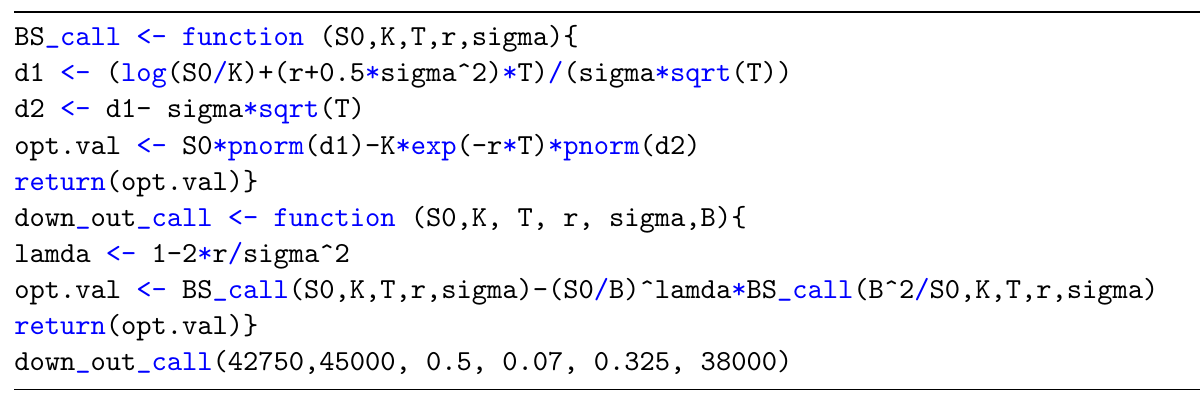
\includegraphics[scale=0.5]{Rcode}
    \end{center}
\end{figure}
\begin{itemize}
\item The final result as $3,018.038$ (VND). \\
\item Compare with the corresponding vanilla call price as $3601.607$ (VND)\\
$\Rightarrow$The barrier option is cheaper $16.2\%$.
\end{itemize}
\end{frame}
\section{Conclusion}
\begin{frame}

{\color{red} \bfseries {Conclusion}}
\begin{itemize}
	\item The pricing formula of European down-and-out call options is derived by using a probabilistic approach\\[0.2cm]
	\item  The application of this formula written on FPT stock
	\item The R code is used as technique to compute the option price
	\item This research will be on the pricing formula of other exotic options
\end{itemize} 
\end{frame}
\begin{frame}
	\begin{figure}[htp]
		\begin{center}
			
\includegraphics[scale=0.8]{fig11}
		\end{center}
	\end{figure}
\end{frame}
\end{document} 